\documentclass[10pt]{article}
%%
%% Language
%%
\usepackage[british,UKenglish]{babel}
\usepackage[utf8]{inputenc}
%%
%% Page size and margins
%%
\usepackage[a4paper,margin=2cm]{geometry}
%%
%% References and style
%%
\usepackage{natbib}
\setcitestyle{aysep={,}}
%%
%% Image and table settings
%%
\usepackage{graphicx}
\graphicspath{{images/}}
\usepackage{multirow}
\usepackage{booktabs}
%%
%% Links - must be last package
\usepackage[pdftex,colorlinks=true,urlcolor=black,citecolor=black,anchorcolor=black,linkcolor=black,filecolor=black]{hyperref}
%%
%% Preamble
%%
\title{Insert the title here}
\author{Insert the author name here}
\date{\today}
%%
\begin{document}
%%
\maketitle
%%
\section{Introduction}
\label{sec:intro}
%%
Include a brief description of this assignment and a paragraph informing the reader of
%%
\section{Assignment 1}
\label{sec:assignment1}
%%
Include in each assignment section, the following items broken down in sub-sections.
%%
\begin{enumerate}
  \item Describe in both non-technical and technical terms the main problem proposed to be solved in the assignment and its main requirements
  \item Briefly describe the main approaches proposed to solve the problem and provide the references to them; if applicable, provide a comparison of the different approaches
  \item Justify descriptively the approach chosen to develop the assignment
  \item Present a brief description of the solution implemented. In case it involves programming code, the commented code shall be released using a version control system.
\end{enumerate}

Below you will find some examples of how to use Figure and Table elements.

Do not forget to include citation to books and other source material in this document. Use \verb|\citep| or \verb|\citet| to cite source material in-text~\citep{author2019}.

Figure~\ref{fig:nci} below is an example of how to insert figures and reference them into the document using \verb|ref{}| command.
%%
\begin{figure}[!th]
  \centering
  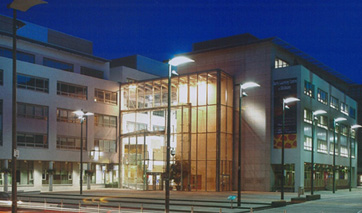
\includegraphics[width=4in]{nci-pic}
  \caption{NCI building.}
  \label{fig:nci}
\end{figure}
%%

Table~\ref{tab:data} shows an example of a table using the \verb|booktabs| and \verb|multirow| packages. More details on how to work with \LaTeX tables can be found at \url{https://en.wikibooks.org/wiki/LaTeX/Tables#Using_booktabs}.
%%
\begin{table}[!th]
\centering
\caption{Some data.}
\label{tab:data}
  \begin{tabular}{llr}
    \toprule
    \multicolumn{2}{c}{Item} &  \\
    \cmidrule(r){1-2}
    Animal    & Description  & Price (\$) \\ \midrule
    Gnat      & per gram     &      13.65 \\
              & each         &       0.01 \\
    Gnu       & stuffed      &      92.50 \\
    Emu       & stuffed      &      33.33 \\
    Armadillo & frozen       &       8.99 \\ \bottomrule
  \end{tabular}
\end{table}
%%
\section{Assignment 2}
\label{sec:assignment2}
%%
Repeat the same items from Section~\ref{sec:assignment1} for Assignment 2.
%%
\section{Assignment 3}
\label{sec:assignment3}
%%
Repeat the same items from Section~\ref{sec:assignment1} for Assignment 3.
%%
%%
%% References
%%
\bibliographystyle{dcu}
\bibliography{references}
%%
\end{document}
%%